\documentclass[11pt]{article}
\usepackage{latexsym}
\usepackage{amsmath}
\usepackage{amssymb}
\usepackage{amsthm}
\usepackage{epsfig}
\usepackage[tight]{subfigure}

\usepackage{amsmath}

\DeclareMathOperator*{\minimize}{min}
\DeclareMathOperator*{\maximize}{max}

\usepackage{algorithm}
 %on linux you may need to run sudo apt-get install texlive-full to install algorithm.sys
% \usepackage{algorithmic}
\usepackage{algpseudocode}
% \algsetup{linenosize=\small}
% \usepackage{algorithm2e,float} % for smaller alg
% \usepackage{algorithm}

\usepackage{verbatim}

% added by yenchi
\usepackage[pagebackref=true,breaklinks=true,letterpaper=true,colorlinks,citecolor=blue,linkcolor=blue,bookmarks=false]{hyperref}
\usepackage{tabularx}
\usepackage{paralist}
\usepackage{booktabs}
\usepackage{xspace} % for \eg, \ie, etc.
\usepackage{stmaryrd}
\usepackage[normalem]{ulem}
\usepackage[tableposition=top]{caption}
\usepackage{appendix}

% for algorithm indent 
\newlength\myindent
\setlength\myindent{2em}
\newcommand\bindent{%
  \begingroup
  \setlength{\itemindent}{\myindent}
  \addtolength{\algorithmicindent}{\myindent}
}
\newcommand\eindent{\endgroup}

% For editing
\usepackage{color}
\definecolor{crimson}{rgb}{0.86, 0.08, 0.24}
\definecolor{gray}{rgb}{0.5,0.5,0.5}
\definecolor{green}{rgb}{0, 0.4, 0}
\definecolor{orange}{rgb}{1, 0.5, 0}
\definecolor{mahogany}{rgb}{0.75, 0.25, 0.0}
\definecolor{purple}{rgb}{0.6, 0, 0.6}
\definecolor{darkgreen}{rgb}{0, 0.4, 0}
\definecolor{frenchblue}{rgb}{0.0, 0.45, 0.73}
\definecolor{red}{rgb}{1,0,0}
\definecolor{yellow}{rgb}{1,1,0}
\definecolor{magenta}{rgb}{1,0,1}
\definecolor{pink}{rgb}{1,0.412,0.706}
\definecolor{newgreen}{rgb}{0, 0.6, 0.2}
\definecolor{blue}{rgb}{0, 0, 1}

\ifx \submission \undefined
% 	\newcommand{\yenchi}[1]{{\color{frenchblue}{#1}}}
	\newcommand{\todo}[1]{({\color{purple}{#1}})}
\else
% 	\newcommand{\yenchi}[1]{{#1}}
	\newcommand{\todo}[1]{{#1}}
\fi

% \newcommand{\norm}[1]{\|#1\|_2}
\newcommand{\norm}[1]{\left\lVert#1\right\rVert}
\newcommand{\dotproduct}[2]{\langle #1 \, ,  #2 \rangle\,}

\newcommand{\name}{Yen-Chi Cheng}
\newcommand{\andrewid}{yenchich}
\newcommand{\question}{\noindent\textbf{Question: }}
\newcommand{\answer}{\noindent\textbf{Answer: }}

\newcommand{\hatyt}{\hat{y}_t}
\newcommand{\yt}{y_t}


\newcommand{\Av}{\mathbf{A}}
\newcommand{\av}{\mathbf{a}}

\newcommand{\Bv}{\mathbf{B}}
\newcommand{\bv}{\mathbf{b}}

\newcommand{\Uv}{\mathbf{U}}
\newcommand{\uv}{\mathbf{u}}

\newcommand{\Pv}{\mathbf{P}}
\newcommand{\pv}{\mathbf{p}}

\newcommand{\Mv}{\mathbf{M}}
\newcommand{\mv}{\mathbf{m}}

\newcommand{\Wv}{\mathbf{W}}
\newcommand{\wv}{\mathbf{w}}

\newcommand{\Xv}{\mathbf{X}}
\newcommand{\xv}{\mathbf{x}}
% uncomment the following def for final draft
% \def \final {}
\ifx \final \undefined
    % \newcommand{\yenchi}[1]{{\color{frenchblue}{YC:#1}}}
    \newcommand{\yenchi}[1]{{\color{frenchblue}{#1}}}
	\newcommand{\haoming}[1]{{\color{orange}{#1}}}
	\newcommand{\todorep}[2]{{\sout{#1}}~{\color{purple}{#2}}}
\else
	\newcommand{\yenchi}[1]{{#1}}
	\newcommand{\haoming}[1]{{#1}}
	\newcommand{\todorep}[2]{{#2}}
\fi


\newcommand{\handout}[5]{
  \noindent
  \begin{center}
  \framebox{
    \vbox{
      \hbox to 5.78in { {#1} \hfill #2 }
      \vspace{4mm}
      \hbox to 5.78in { {\Large \hfill #5  \hfill} }
      \vspace{2mm}
      \hbox to 5.78in { {\em #3 \hfill #4} }
    }
  }
  \end{center}
  \vspace*{4mm}
}

\newcommand{\lecture}[5]{\handout{#1}{#2}{#3}{#4}{#5}}
\newcommand{\collision}[0]{\mathrm{collision}}
\newcommand{\nocollision}[0]{\overline{\collision}}

\newcommand*{\QED}{\hfill\ensuremath{\square}}

\newtheorem{theorem}{Theorem}
\newtheorem{corollary}[theorem]{Corollary}
\newtheorem{lemma}[theorem]{Lemma}
\newtheorem{observation}[theorem]{Observation}
\newtheorem{proposition}[theorem]{Proposition}
\newtheorem{definition}[theorem]{Definition}
\newtheorem{claim}[theorem]{Claim}
\newtheorem{fact}[theorem]{Fact}
\newtheorem{assumption}[theorem]{Assumption}
\newtheorem{note}[theorem]{Note}

% 1-inch margins, from fullpage.sty by H.Partl, Version 2, Dec. 15, 1988.
\topmargin 0pt
\advance \topmargin by -\headheight
\advance \topmargin by -\headsep
\textheight 8.9in
\oddsidemargin 0pt
\evensidemargin \oddsidemargin
\marginparwidth 0.5in
\textwidth 6.5in

\parindent 0in
\parskip 1.5ex
%\renewcommand{\baselinestretch}{1.25}

%%% DISCLAIMER: we reference some of the content from Spring 2020's scribe note: https://www.dropbox.com/sh/j92mhvfeukmuz2f/AABTdMvmDghIx98YTBW9XMI1a?dl=0&preview=Lecture_4_PWEA_RWMA__OLC_Perceptron.pdf
%%% Some other reference:
%   - https://en.wikipedia.org/wiki/Winnow_(algorithm)
%   - https://en.wikipedia.org/wiki/Perceptron

\begin{document}

\lecture{Statistical Techniques in Robotics (16-831, S21)}{Lecture \#14
  (Wednesday, March 24)}{Lecturer: Kris Kitani}{Scribes: Yen-Chi Cheng, Hao-Ming Fu}{EXP3, EXP4}

\vspace{-10mm}
\section{Review}
\vspace{-5mm}
% \subsection{Weighted Majority Algorithm (WMA)}
\normalfont
In the last lecture, we talked about the Thompson Sampling~\cite{thompson1933likelihood} in the stochastic multi-armed bandits problem. In this setting, we assume that each reward is drawn from a parametrized distribution $r \sim p(r | a, \theta)$. If the true parameters for the likelihood function are known, our best action to pull the arm is
$$
 a = \mathrm{arg} \max_k \mathbb{E}_{p(r | a_k, \theta_k^{*}) [ r | a_k, \theta_k^{*}]}
$$
but often the true parameters are unknown, so we approximate it with the posterior distribution
\begin{equation}
     \hat{\theta} = \mathrm{arg} \max_{\theta} p (\theta | h^{(t)} = (a^{(1)}, r^{(1)}, \ldots, a^{(t)}, r^{(t)}) )
     \label{eq:posterior}
     \vspace{-1mm}
\end{equation}
where $h^{(t)}$ is the history. To model the posterior distribution, we apply the Bayes' Rule:
\vspace{-1mm}
\begin{align*}
    p(\theta | a^{(1)}, r^{(1)}, \ldots, a^{(t)}, r^{(t)} ) &= \frac{\prod_t p(r^{(t)} | a^{(t)}, \theta) p(\theta)}{\prod_t p(r^{(t)}) | a^{(t)}) }\,  \\
    &\propto \prod_t p(r^{(t)} | a^{(t)}, \theta) p(\theta)\, \hspace{45pt} \text{by Markov Assumption} \\
    &\propto p(r^{(t)} | a^{(t)}, \theta) p(\theta | h^{(t-1)})\, \hspace{20pt} \text{writing the posterior recursively}
\end{align*}
Now back to the original problem, the Equation~\ref{eq:posterior} becomes:
\vspace{-1mm}
\begin{align*}
    \hat{\theta}_k = \mathrm{arg} \max_{\theta_k} p(r^{(t)} | a_k^{(t)}, \theta_k) p(\theta_k | h_k^{(t-1)})
\end{align*}
\vspace{-.5mm}
To update the parameter efficiently, we adopt the conjugate priors: given that the Beta distribution is the conjugate prior of the Bernoulli, the update equation w.r.t a single arm is
\begin{align*}
    p(\theta | h^{(t)}) &\propto p(r^{(t)} | a_k^{(t)}, \theta_k) p(\theta_k | h_k^{(t-1)})\, \\
    &\propto \theta^r (1-\theta)^{(1-r)} \theta^{(\alpha -1)} (1-\theta)^{(\beta - 1)}\, \\
    &\propto \theta^{(r+\alpha)-1} (1-\theta)^{(1-r+\beta)-1}\, \\
    &\propto \theta^{\alpha^{\prime}-1} (1-\theta)^{\beta^{\prime}-1}
\end{align*}
\vspace{-.5mm}
The algorithm is listed at Alg.~\ref{algo:thompson}.
And the regret of the Thompson Sampling is \\ $BR(T) = O (\sqrt{KT \log T})$.
% \vspace{-.5mm}
% $$
% BR(T) = O (\sqrt{KT \log T})
% $$
% \vspace{-.5mm}
% \small{
\begin{algorithm}[H]
\small
\caption{Thompson Sampling.}
\label{algo:thompson}
\begin{algorithmic}[1]
\Function{Thompsons Sampling }{}
% \State $\pmb{w}^{(1)} \leftarrow \{w_k^{(1)} \}_{k=1}^{K}$ \hfill $\triangleright$ weights over actions
\For{$t=1,\;\cdots,\;T$}
\State $\theta_k \sim p(\theta_k | h_k^{(t^{\prime})})$ \,\,\, $\forall k$ \hfill $\triangleright$ sample from posterior
\State $a_{\hat{k}}^{(t)} = \mathrm{arg} \max_k \mathbb{E}_{p(r | a_k, \theta_k)} [r | a_k, \theta_k] $ \hfill $\triangleright$ predict
\State \textsc{Receive}$ (r^{(t)})$ \hfill $\triangleright$ get sampled reward
\State $h_{\hat{k}}^{(t^{\prime} + 1)} = h_{\hat{k}}^{t^{\prime}} \bigcup (r^{(t)}, a_{\hat{k}}^{(t)} )$ \hfill $\triangleright$ update history
\State $p(\theta_{\hat{k}} | h_{\hat{k}}^{(t^{\prime} + 1)} ) \propto p(h_{\hat{k}}^{(t^{\prime} +1)} | \theta_{\hat{k}} )  p( \theta_{\hat{k}} | h_{\hat{k}}^{(t^{\prime} +1)}) $ \hfill $\triangleright$ update posterior
\EndFor
% \STATE \textbf{end}
\EndFunction

\end{algorithmic}
\end{algorithm}


\clearpage

%%%%%%

% \section{Summary for Lecture \#05}
\section{EXP3}
% \label{ssec:online_linear_cls}
\subsection{Overview}

EXP3~\cite{auer2002nonstochastic} is a multi-armed bandit problem in an adversarial environment setting. The environment could observe the agents' actions and decides the payoff structure based on it. The adversarial setting is one of the strongest generalizations of the bandit problem. Unlike the stochastic environment, it removes all the assumptions of the reward followings a certain distribution and thus provides a more generalized solution. The EXP3 stands for \textbf{Exp}onential-Weight Update algorithm for \textbf{Exp}loration and \textbf{Exp}loitation. Different types of bandits are listed at Table~\ref{tab:bandits}.
% The difference between EXP3 and previous algorithms could be seen in the following paradigm (see Fig.~\ref{fig:paradigm}).

% \begin{figure}
%     \centering
%     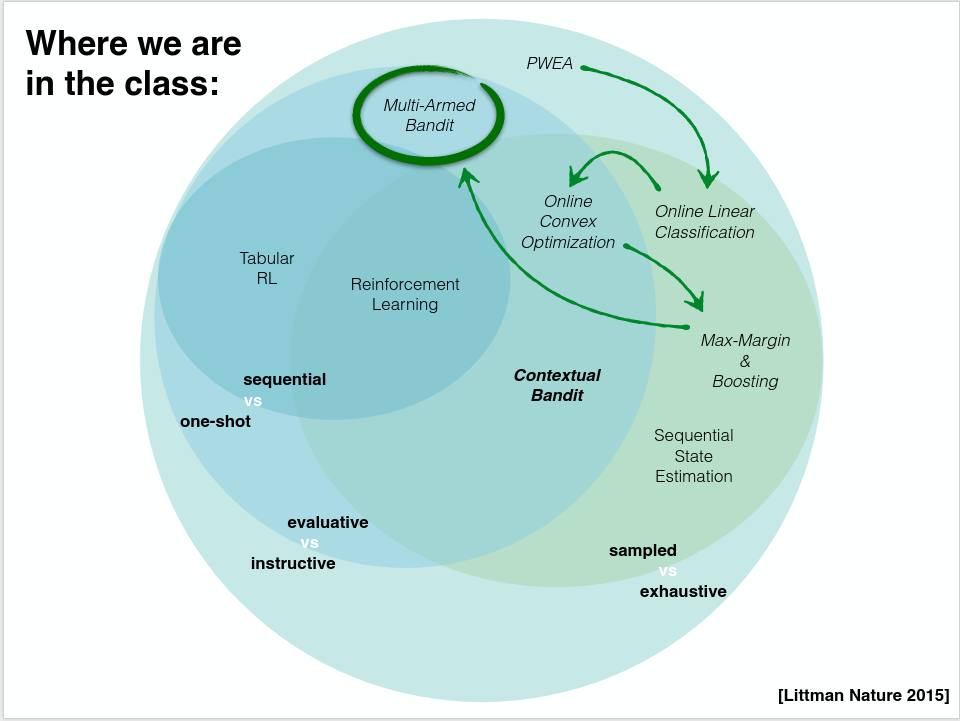
\includegraphics[width=\linewidth]{img/paradigm.png}
%     \caption{Paradigm.}
%     \label{fig:paradigm}
% \end{figure}

The algorithm is listed at Algorithm~\ref{algo:exp3}. One can notice that EXP3 algorithm is very similar to the Hedge algorithm. The differences are as follows:
\begin{itemize}
    \item EXP3 do not have the \textit{expert advice}.
    \item We receive \textit{partially observable reward}, while in the Hedge algorithm, the true label is revealed.
    \item The loss is known for \textit{one} expert, and could only update \textit{one} weight, while the hedge algorithm could update all weights since the loss is known for all hypothesis.
\end{itemize}

\begin{table}[h]
    \centering
    \begin{tabular}{r  c  c}
    \toprule
            & \textbf{Context-free} & \textbf{Contextual} \\
    \midrule
    \textbf{Stochastic environment}  & Explore-Exploit, UCB, Thompson Sampling & linUCB\\
    \textbf{Adversarial environment} & \textbf{EXP3} & \textbf{EXP4}\\
    \bottomrule
    \end{tabular}
    \caption{Types of bandits}
    \label{tab:bandits}
\end{table}

\begin{algorithm}[H]
\caption{EXP3 Algorithm}
\label{algo:exp3}
\begin{algorithmic}[1]
\Function{EXP3}{$\gamma \in [0, 1]$}
\State $\pmb{w}^{(1)} \leftarrow \{w_k^{(1)} \}_{k=1}^{K}$ \hfill $\triangleright$ weights over actions
\For{$t=1,\;\cdots,\;T$}
\State $\pmb{p}^{(t)} = \frac{\pmb{w}^{(t)}}{\sum_k w_k^{(t)}}$ \hfill $\triangleright$ probability over actions
\State $k \sim $\textsc{Multinomial}$(\pmb{p}^{(t)})$ \hfill $\triangleright$ take and draw action
\State $a^{(t)}=a_k$
\State \textsc{Receive} ($r^{(t)}\in [0, 1]$) \hfill $\triangleright$ get reward
\State $w_{k}^{(t+1)}\leftarrow w_{k}^{(t)} \exp{(\gamma \cdot r^{(t)}/p_k^{(t)})}$ \hfill $\triangleright$ update weights
\EndFor
% \STATE \textbf{end}
\EndFunction
\end{algorithmic}
\end{algorithm}


\subsection{The Unbiased Estimator}

In line 8 of the Algorithm~\ref{algo:exp3}, we notice an mysterious update term $r^{(t)}/p_k^{(t)}$. The re-weighting is the sampling strategy to make the sampled reward an \textit{unbiased estimator}. To understand this, we discuss two cases below:
\begin{itemize}
    \item \textbf{Case 1: Single-arm stochastic bandit.} To estimate the true mean $\mu_t$, we sampled the reward and compute the empirical mean reward by defining the following estimator:
    \begin{align*}
        c_1^{(t)}(a^{(t)}) = \mathbf{1} [a^{(t)} = 1] \cdot r^{(t)}\, . \\
    \end{align*}
    where $c_1^{(t)}$ denotes the first arm at time $t$. And the expected value of $ c_1^{(t)}(a^{(t)}) $ at time $t$ is
    \begin{align*}
        \mathbb{E}_{p(a)} \left[  c_1^{(t)}(a^{(t)}) \right] &= p (a^{(t)} = 1) \cdot \mathbf{1} [a^{(t)} = 1] \cdot r^{(t)} \, , \\
        &= r^{(t)}\, .
    \end{align*}
    The expected value of the estimator over $\textit{T}$ round:
    \begin{align*}
        \mathbb{E}_{p(a)} \left[ \frac{1}{T} \sum_{t=1}^{T} c_1^{(t)}(a^{(t)}) \right] &= \frac{1}{T} \sum_{t=1}^{T} r^{(t)} \, .
    \end{align*}
    which is the empirical estimate of the true mean $\mu_t$.
    \item \textbf{Case 2: Two-arm stochastic bandit}. In this case, we could select action from two arms with a probability distribution $(50/50)$. We again compute the empirical mean for arm 1 as follows:
    \begin{align*}
        c_1^{(t)}(a^{(t)}) = \mathbf{1} [a^{(t)} = 1] \cdot r^{(t)}\, , \\
        c_2^{(t)}(a^{(t)}) = \mathbf{1} [a^{(t)} = 2] \cdot r^{(t)}\, . \\
    \end{align*}
    where $c_k$ denotes $k_{th}$ arm, $k = 1, 2.$ And the expected value of the estimator is
    \begin{align}
        \mathbb{E}_{p(a)} \left[  c_1^{(t)}(a^{(t)}) \right] &= p (a^{(t)} = 1) \cdot c_1^{(t)}(1) + p (a^{(t)} = 2) \cdot c_1^{(t)}(2)\, , \nonumber \\
        &= p (a^{(t)} = 1) \cdot  \mathbf{1} [a^{(t)} = 1] \cdot r^{(t)} + p (a^{(t)} = 2) \cdot \mathbf{1} [a^{(t)} = 1] \cdot r^{(t)} \, ,  \nonumber \\
        &= (0.5) \cdot 1 \cdot r^{(t)} + (0.5) \cdot 0 \cdot r^{(t)}\, , \nonumber \\
        &= (0.5) \cdot r^{(t)}\, .
        \label{eq:reward_half}
    \end{align}
    here we are getting a scaled reward back. We continue to compute the expected value of the estimator over T round:
    \begin{align*}
        \mathbb{E}_{p(a)} \left[ \frac{1}{T} \sum_{t=1}^{T} c_1^{(t)} (a^{(t)}) \right] = \frac{1}{T} \sum_{t=1}^{T} (0.5) r^{(t)}\, .
    \end{align*}
    and we found that the reward is multiplied by the probability of that arm. To fix this, \textit{inverse probability weighting} or \textit{importance sampling} is proposed to address this problem.
\end{itemize}

\subsection{Inverse Probability Weighting}
Recall Equation~\ref{eq:reward_half}, the expected value of the estimator is scaled down by $0.5$. To fix that, we multiply the term by \textit{the inverse of the probability of selecting that arm} (which is $\frac{1}{p_1} = 2$):
\begin{align*}
    c_1^{(t)}(a^{(t)}) = \mathbf{1}[a^{(t)}=1] \cdot r^{(t)} \cdot \frac{1}{p_1}\, , \\
\end{align*}
and the expected value of the estimator becomes
\begin{align*}
    \mathbb{E}_{p(a)} \left[ c_1^{(t)} (a^{(t)})\right] &= p(a^{(t)} = 1) \cdot c_1^{(t)} (1) + p(a^{(t)} = 2) \cdot c_1^{(t)} (2)\, , \\
    &= p(a^{(t)} = 1) \mathbf{1}[a^{(t)} = 1] \cdot r^{(t)} \cdot \frac{1}{p_1} + p(a^{(t)} = 2) \mathbf{1}[a^{(t)} = 1] \cdot r^{(t)} \cdot \frac{1}{p_1}\, , \\
    &= (0.5) \cdot 1 \cdot r^{(t)} \cdot \frac{1}{0.5} + (0.5) \cdot 0 \cdot r^{(t)} \cdot \frac{1}{0.5}\, , \\
    &= r^{(t)}\, .
\end{align*}
so the expected value is the reward value, and the estimator becomes the unbiased estimator to the true mean $\mu_t$. In general, the unbiased estimator for the expected reward of $k_{th}$ arm, given that the probability of selecting it equals $p_k$, is
\begin{align*}
    c_k^{(t)}(a^{(t)}) &= \mathbf{1}[a^{(t)}=k] \cdot r^{(t)} \cdot \frac{1}{p_k}\, , \,\,\, \forall k\, , \\
    \mathbb{E}\left[ c_a^{(t)} (a^{(t)}) \right] &= \sum_{k=1}^{K} p_k \cdot \mathbf{1} [a^{(t)} = a] \cdot r^{(t)} \cdot \frac{1}{p_k}\, , \\
    &= p(a^{(t)} = a) \cdot r^{(t)} \cdot \frac{1}{p_a}\, , \\
    &= r^{(t)}\, .
\end{align*}
Therefore the mysterious term in line 8 of the Algorithm~\ref{algo:exp3}, is the unbiased estimator to the true mean $\mu_t$. Now let's discuss the behavior of the update equation:
\begin{align*}
    w_k^{(t+1)} = w_k^{(t)} \exp{\{\gamma \cdot r^{(t)}/p_k^{(t)} )\}}
\end{align*}
Given the reward $r^{(t)}$ and the probability $p_k^{(t)}$, the behaviors of the agent are listed at Table~\ref{tab:behavior}
\begin{table}[h]
    \centering
    \begin{tabular}{c  c  c}
    \toprule
    \textbf{Reward} $r$        & \textbf{Probability} p & \textbf{Results in...} \\
    \midrule
    huge  & tiny & Exploitation\\
    small  & tiny & Exploration\\
    0 & moderate & unchanged\\
    \bottomrule
    \end{tabular}
    \caption{\textit{Exploration} or \textit{Exploitation}?}
    \label{tab:behavior}
\end{table}


% \begin{figure}[H]
%     \centering
%     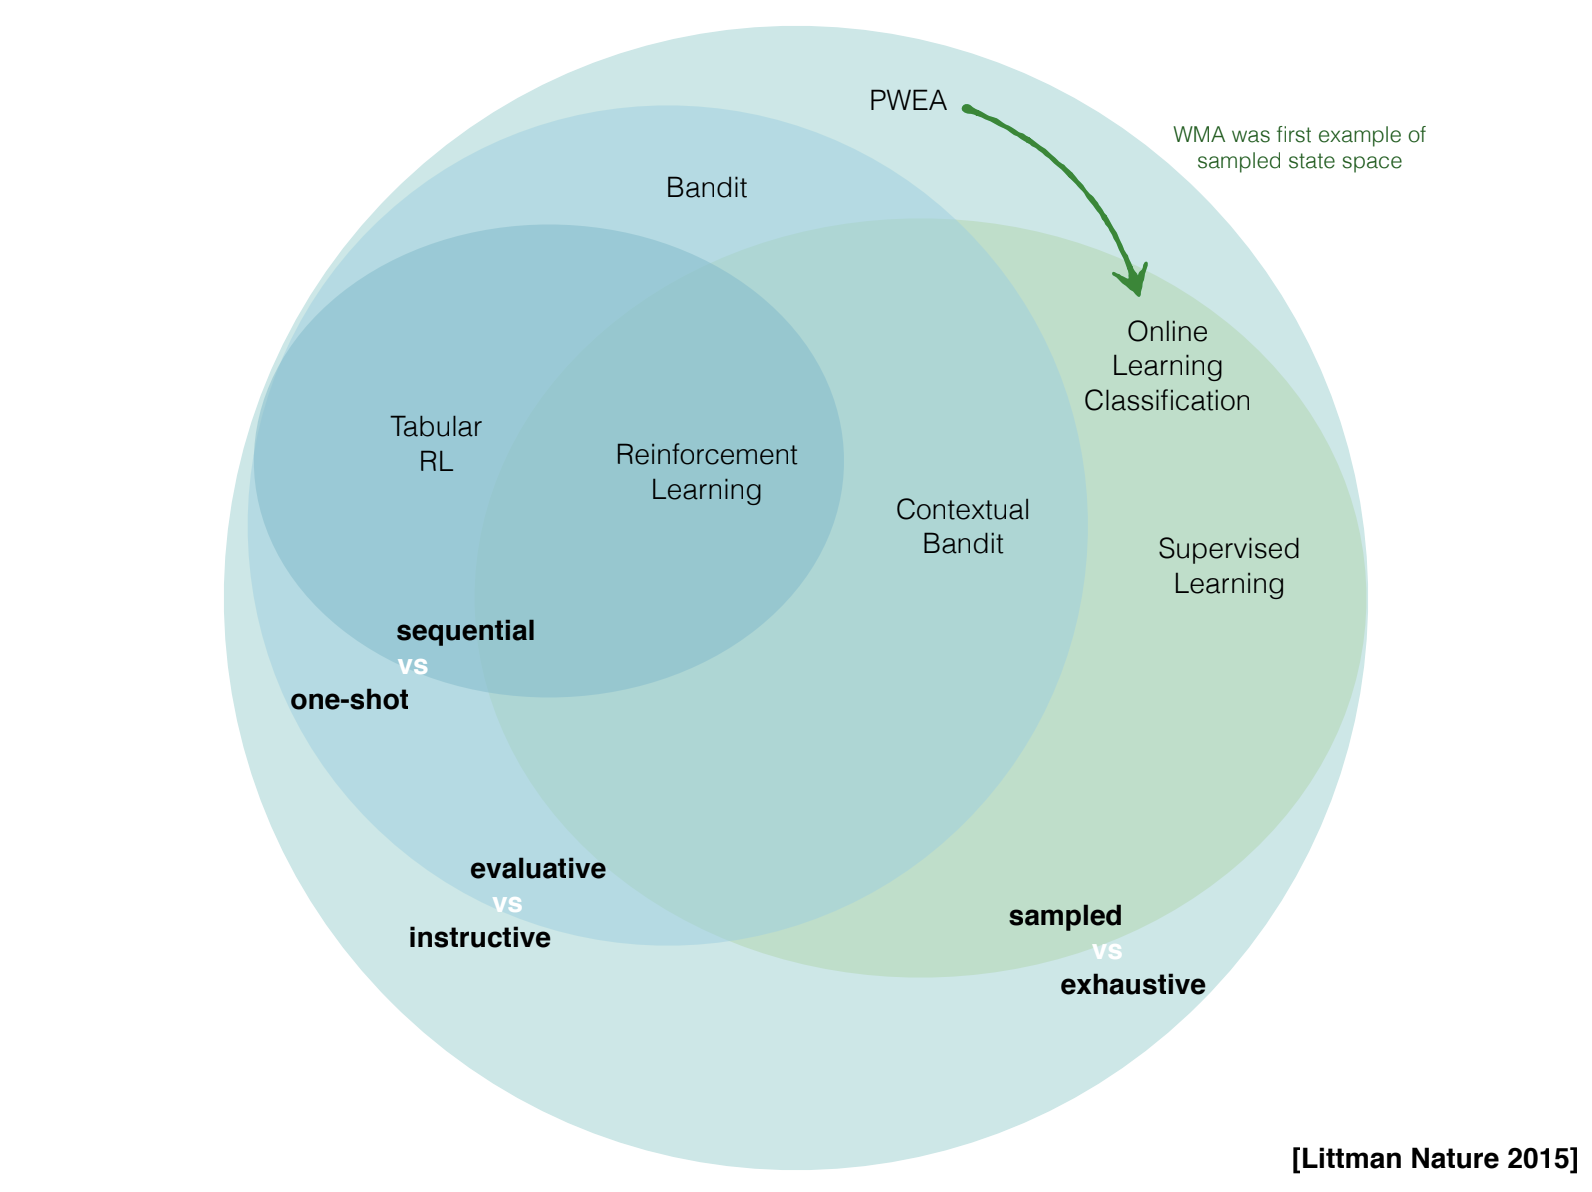
\includegraphics[width=\linewidth]{img/diagram.png}
%     \caption{Caption}
%     \label{fig:my_label}
% \end{figure}

\subsection{Regret Bound}

Now we try to bound the regret for the EXP3 algorithm. As usual, we first properly define a potential function that assists our mathematical calculation. Then, we finds the upper and lower bounds of the potential function. Finally, we combine the inequalities and apply some basic algebra to derive the regret bound.

First, for convenience, we define $z^{(t)}$ as the sum of the weights $w$ of all $k$ bandits at time $t$:
\begin{align}
    z^{(t)} = \sum_{k}w^{(t)}_k
\end{align}
With this, now we define the potential function $\Phi()$ as the sum of log difference of $z^{(t)}$ overall all time steps until time $T$:
\begin{align}
    \Phi = \sum_{t=1}^T log(\frac{z^{(t+1)}}{z^{(t)}})
\end{align}
Then, we calculate the upper bound of this potential function $\Phi$. By inserting the definition of $z$ into that of $\Phi$, we have:
\begin{align}
    \Phi = \sum_{t=1}^T log(\frac{z^{(t+1)}}{z^{(t)}}) = \sum_{t=1}^T log(\frac{\sum_{k}w^{(t+1)}_k}{\sum_{k'}w^{(t)}_{k'}})
\end{align}
Assuming that we are dealing with a single known sequence, recall that from time $t$ to $t+1$, we update each weight $w$ by multiplying it with an exponential term that conditions on the gain $g$ of each bandit. Thus, we can get this:
\begin{align}
    \Phi = \sum_{t=1}^T log(\frac{\sum_{k}w^{(t)}_k exp(\gamma \cdot g_k^{(t)})}{\sum_{k'}w^{(t)}_{k'}}) = \sum_{t=1}^T log(\sum_{k} \frac{w^{(t)}_k }{\sum_{k'}w^{(t)}_{k'}} exp(\gamma \cdot g_k^{(t)}))
\end{align}
Notice that the fractional term with $w$ is actually the probability of sampling the $k^{th}$ bandit, $p_k$, according to the algorithm. So, we can replace the term with $p$ and obtain:
\begin{align}
    \Phi = \sum_{t=1}^T log(\sum_{k} p_k^{(t)} exp(\gamma \cdot g_k^{(t)}))
\end{align}
To replace the exponential term with a polynomial one, we apply the inequality $e^x \leq 1 + x + x^2$ and obtain:
\begin{align}
    \Phi \leq \sum_{t=1}^T log(\sum_{k} p_k^{(t)} (1 + \gamma \cdot g_k^{(t)} + (\gamma \cdot g_k^{(t)})^2))
\end{align}
By distributing $\sum_{k}p_k^{(t)}$ into each of the terms, we obtain:
\begin{align}
    \Phi \leq \sum_{t=1}^T log( \sum_{k}p_k^{(t)} + \sum_{k}p_k^{(t)}\gamma \cdot g_k^{(t)} + \sum_{k}p_k^{(t)}(\gamma \cdot g_k^{(t)})^2)
\end{align}
Knowing that the selection probabilities of each bandit should sum to $1$ and the inequality $log(x+1) \leq x$, we have
\begin{align}
    \Phi \leq \sum_{t=1}^T log( 1 + \sum_{k}p_k^{(t)}\gamma \cdot g_k^{(t)} + \sum_{k}p_k^{(t)}(\gamma \cdot g_k^{(t)})^2)\\
    \leq \sum_{t=1}^T (\sum_{k}p_k^{(t)}\gamma \cdot g_k^{(t)} + \sum_{k}p_k^{(t)}(\gamma \cdot g_k^{(t)})^2)
\end{align}
This is the upper bound of the potential function. Now, we calculate its lower bound. We represent $\Phi$ as the log movement of $z$ from its initial value $K$:
\begin{align}
    \Phi = log(\frac{z^{(T+1)}}{z^{(1)}}) = log(\frac{z^{(T+1)}}{K})
\end{align}
Inserting the definition of $z$ and considering the update of $w$ from its initial value 1, we have:
\begin{align}
    \Phi = -logK + log\sum_{k=1}^{K}w_k^{(T+1)} \\
    = -logK + log\sum_{k=1}^{K}\prod_{t=1}^T exp(\gamma \cdot g_k^{(t)})\\
    = -logK + log\sum_{k=1}^{K} exp(\gamma \cdot \sum_{t=1}^T g_k^{(t)})
\end{align}
As the gain $g$ is always positive, we can arbitrarily pick any $k$ and obtain the inequality:
\begin{align}
    \Phi \geq -logK + log( exp(\gamma \cdot \sum_{t=1}^T g_k^{(t)})) \quad \forall k \\
    = -logK + \gamma \cdot \sum_{t=1}^T g_k^{(t)} \quad \forall k
\end{align}
This is the lower bound of the potential function. Finally, we combine the upper and the lower bounds:
\begin{align}
    -logK + \gamma \cdot \sum_{t=1}^T g_j^{(t)} \leq \sum_{t=1}^T (\sum_{k}p_k^{(t)}\gamma \cdot g_k^{(t)} + \sum_{k}p_k^{(t)}(\gamma \cdot g_k^{(t)})^2) \quad \forall j
\end{align}

Notice that we change the index $k$ in the lower bound to $k$ to avoid the conflict with the summation index $k$ in the upper bound. Now, rather than let the inequality hold for all bandits $j$, we select the one with the maximum gain to obtain the strongest statement among these options. This help us get rid of the $\forall j$ statement. Also, with some algebraic operations, we obtain
\begin{align}
    \max_j \sum_{t=1}^T g_j^{(t)} - \sum_{t=1}^T \sum_{k=1}^K p_k^{(t)} g_j^{(t)} \leq \frac{logK}{\gamma} + \sum_{t=1}^T \sum_{k=1}^K p_k^{(t)} \cdot \gamma (g_k^{(t)})^2
\end{align}
Notice that the first term on the left hand side is the total gain of the best bandit and the second term is the performance of the EXP3 algorithm. Combining these, the left hand side of the inequality is the regret of EXP3, which gives us the upper bound of the regret of EXP3.

This result is obtained from a specific sequence of actions and a certain sampled reward from the adversarial world. To make the regret bound general, we have to calculate the expected value of regret rather than that of a certain sequence. Take the expectation for the both sides:
\begin{align*}
    E(\textbf{regret}) &= R^{(T)} \leq E( \frac{logK}{\gamma} + \gamma \sum_{t=1}^T \sum_{k=1}^K p_k^{(t)} \cdot (g_k^{(t)})^2 ) \\
    &\leq \frac{logK}{\gamma} + \gamma \sum_{t=1}^T E( \sum_{k=1}^K p_k^{(t)} \cdot (g_k^{(t)})^2 )\\
    &= \frac{logK}{\gamma} + \gamma \sum_{t=1}^T E(p_{k^{(t)}}^{(t)} \cdot (\frac{r^{(t)}}{p_{k^{(t)}}^{(t)}})^2 ) = \frac{logK}{\gamma} + \gamma \sum_{t=1}^T E(\frac{(r^{(t)})^2}{p_{k^{(t)}}^{(t)}})\\
    &\leq \frac{logK}{\gamma} + \gamma \sum_{t=1}^T E(\frac{1}{p_{k^{(t)}}^{(t)}}) = \frac{logK}{\gamma} + \gamma \sum_{t=1}^T K = \frac{logK}{\gamma} + \gamma T K
\end{align*}
Finally, we can observe that when $\gamma$ goes to infinity or negative infinity, the bound explodes. As a result, we can find the $\gamma$ that leads to the smallest upper bound by requiring the derivative of the bound to be zero:
\begin{align}
    \frac{d}{d\gamma}(\frac{logK}{\gamma} + \gamma T K) = 0\\
    \implies -\frac{logK}{\gamma^2} + T K = 0\\
    \implies \gamma^2 = \frac{logK}{TK}\\
    \implies \gamma = \sqrt{\frac{logK}{TK}}
\end{align}
Now we have the $\gamma$ that minimizes the upper bound of regret. We then calculate the corresponding upper bound by inserting this $\gamma$ into the bound:
\begin{align}
    R \leq \frac{logK}{\sqrt{\frac{logK}{TK}}} + \sqrt{\frac{logK}{TK}} TK\\
    = 2\sqrt{TKlogK}
\end{align}
This means that with a big O notation,
\begin{align}
    R = O(\sqrt{TKlogK})
\end{align}
This shows that the regret is sublinear to $T$, meaning that EXP3 is a no regret algorithm.
\section{EXP4}
The EXP4 algorithm, Exponential-Weighted Update algorithm for Exploration and Exploitation with Experts, is similar to the EXP3 algorithm in many ways. The major difference is that EXP4 learns weights for each experts providing advises for pulling the bandits rather than learning weights for each bandit directly. This is the algorithm of EXP4:

\begin{algorithm}[H]
% \algsetup{linenosize=\tiny}
\caption{EXP4 Algorithm}
\label{algo:exp4}
\begin{algorithmic}[1]
\Function{EXP4}{$\gamma \in [0, 1], T$}
\State $\pmb{w}^{(1)} \leftarrow 1 \in R^N$ \hfill $\triangleright$ weights over experts
\For{$t=1,\;\cdots,\;T$}
\State \textsc{Receive} ($\pmb{X}^{(t)}\in R^{N \times K}$) \hfill $\triangleright$ advice from N experts
\State $\pmb{q}^{(t)} = \frac{\pmb{w}^{(t)}}{||\pmb{w}||^2} \cdot \pmb{X}^{(t)} \in \Delta^K$ \hfill $\triangleright$ probability over actions
\State $k^{(t)} \sim $\textsc{Multinomial}$(\pmb{q}^{(t)})$ \hfill $\triangleright$ draw action
\State \textsc{Receive} ($r^{(t)}$) \hfill $\triangleright$ get reward
\State $\pmb{\hat{r}}^{(t)} = \frac{r^{(t)}}{q^{(t)}_k} I [k = k^{(t)}] \in I^K$ \hfill $\triangleright$ reward over all arms
\State $\pmb{g}^{(t)} = \pmb{X}^{(t)} \cdot \pmb{\hat{r}}^{(t)} \in R^N $ \hfill $\triangleright$ per expert reward
\State $w_{n}^{(t+1)}\leftarrow w_{n}^{(t)} \exp{(\gamma \cdot g_n^{(t)})} \quad \forall n$ \hfill $\triangleright$ update
\EndFor
% \STATE \textbf{end}
\EndFunction
\end{algorithmic}
\end{algorithm}

From the algorithm we can observe the major differences lie in line 5 and line 10, where the probability distribution over actions are replaced by that over experts and weights for experts rather than actions are updated. \\
Through similar derivation process for EXP3, we can obtain that the regret bound of EXP4 has a similar form with that of EXP3.
\begin{align}
    R_{EXP3} \leq \sqrt{KTlogK}\\
    R_{EXP4} \leq \sqrt{KTlogN}
\end{align}
Note that the $logK$ is now replaced by $logN$ because the number of weights has changed from the number of bandits (actions) $K$ to that of experts $N$.

\vspace{-5mm}
\section{Conclusion}
\vspace{-3mm}
In this lecture, we discuss a more generalized setting in the multi-armed bandits problem: the adversarial environment. The EXP3 algorithm is proposed to solve this problem. The algorithm is similar to the Hedge algorithm we learned before, but there is no expert advises and the loss is only known to one action, and we could only update one weight. In the update equation of the EXP3 algorithm, the Inverse Probability Weighting is incorporated to make the true mean estimator $c_k^{(t)}(a^{(t)})$ an unbiased estimator. The update equation in EXP3 will make the agent to \textit{explore} more if the sampled reward is small, and \textit{exploit} if the sampled reward is huge.

Then we tried to obtain an upper bound for its regret. As always, we defined a potential function for which we can find an upper bound and a lower bound. Finally, we combine the two bounds and obtain the upper bound of regret. As $\gamma$ is a hyper parameter that we can design, we found the $gamma$ that minimizes the regret bound. With such $\gamma$, the upper bound of regret is sublinear with regard to time steps $T$ and thus EXP3 is a no regret algorithm.

As for EXP4, knowing that it is quite similar to EXP3, we noticed that their major difference is that each of the weights in EXP3 corresponds to an action, while that in EXP4 corresponds to an expert. Accordingly, we also derived the regret bound for EXP4.

%\todo{EXP3 is a no-regret algorithm. Write some conclusion of EXP4}

% The goal of the online learning classification is for the autonomous system, where experts will work along side and give the `correct' classification. It aims to facilitate the autonomous system to learn a good classifier over time. We covered two online learning classification algorithm: the Perceptron Algorithm and the Winnow Algorithm. The Perceptron Algorithm adopted additive approach for its update rule. It is fast in both aspect of prediction and update, but have no notion of regret. Assuming linear separability, the number of mistakes will converge. On the other hand, the Winnow Algorithm uses multiplicative rule for updating the weight, and is adopted to learn the logical OR function of $k$ relevant attributes. 

%\section*{References}
%Include your references here. Please cite any resources you found useful.	
%Populate the refs.bib file or list your references manually. Be consistent in formatting!
{
\bibliography{refs}
\bibliographystyle{abbrv}
}

%\section{Appendix}
%This section provides any relevant background material that was not covered in the lectures, but was found to be useful for understanding the material. 
%For example, derivations, theory underlying techniques employed, etc. 

%Additionally, this section can summarizes applications or extensions of these techniques found in the literature. 


\clearpage

% \begin{appendix}

% \section{AAA}

% \end{appendix}


\end{document} % Done!


